\chapter{The Embedding Problem: Theoretical Framework} \label{chap:embedding_problem}

This chapter introduces the theoretical framework behind the embedding problem for Neutral Atom Quantum Architectures. 
The aim of this part is to explain the complexity of finding efficient embeddings, starting with an introduction of basic concepts 
of computational complexity and graph theory, and then proceed to define Unit Disk Graphs (UDG) and the Maximum Independent Set (MIS) problem. Finally, these concepts will be connected to the current State of the Art (SOTA) and the Quadratic Unconstrained Binary Optimization (QUBO) formulation.


\section{Combinatorial Optimization and Computational and Geometrical Complexity}
\label{sec:combinatorial_opti_def}


Combinatorial optimization is a prominent branch of applied mathematics and computer science that focuses on finding an optimal object from a finite, discrete set of possible solutions. Specifically, the objective is to identify a solution that minimizes (or maximizes) a well-defined cost function, often subject to a set of strict mathematical constraints \cite{korte2012combinatorial}. 

These problems commonly involve discrete mathematical structures such as graphs, permutations, or boolean variables and are ubiquitous in fields ranging from logistics and network routing to machine learning and quantum physics \cite{papadimitriou1998combinatorial}. Although the solution space for these problems can be strictly finite, the number of possible configurations still can be overwhelmingly large. 

Moreover, combinatorial optimization frequently encounters $NP$-Hard problems, where finding the exact global optimum becomes computationally intractable. Consequently, the field heavily leverages heuristics and metaheuristics to find high-quality approximate solutions within a reasonable timeframe. Within this computationally demanding landscape, Quantum Computing emerges as a disruptive paradigm; by exploiting quantum mechanical phenomena, it promises to solve significantly larger $NP$-Hard instances and achieve higher-quality approximate solutions more efficiently than classical approaches \cite{memon2024quantum}.

Provided this general computational complexity, a secondary, equally formidable challenge arises when utilizing neutral atom platforms: the geometrical complexity. As introduced in Chapter \ref{chap:introduction}, executing an embedding algorithm requires mapping (or \textit{embedding}, precisely) the logical variables of the optimization problem onto the physical atoms arranged in a 2D or 3D register \cite{Henriet2020quantumcomputing}. 
In our specific case, focusing on a 2D plane, the hardware imposes strict geometric constraints and specific interaction boundaries governed by the Ising model and the Rydberg blockade. Finding an efficient spatial mapping that preserves the problem's theoretical connectivity while respecting these strict physical limitations is, remarkably, an $NP$-Hard problem in itself \cite{Vercellino_2022}.

\section{Unit Disk Graphs (UDG) and the Maximum Independent Set (MIS)}
\label{sec:UDG_and_MIS}

A graph can be formally denoted as:

\begin{equation}
    G = (V, E)
\end{equation}

where $V$ is the set of vertices (or nodes) and $E$ is the set of edges connecting them. Graphs are very common mathematical structures used to model relations between objects, and their properties are supported by a vast, historically established and robust theoretical foundation \cite{berge2001theory}. 

Thus, while an exhaustive review of graph theory is beyond the scope of this work, these structures will be briefly presented because of fundamental interest. Indeed, a significant portion of current literature focuses on graph-based combinatorial problems, primarily because graphs serve as the standard mathematical interface to encode and map optimization tasks onto quantum architectures. 
Prominent examples of such $NP$-Hard problems include the Maximum Cut (Max-Cut), the Traveling Salesperson Problem (TSP), and the Maximum Independent Set (MIS), which have extensively served as standard benchmarks for evaluating the performance of quantum algorithms \cite{lucas2014ising}.

To specialize our focus from general graphs, we introduce the concept of Unit Disk Graphs (UDG). As formalized by Clark et al. \cite{CLARK1990165}, UDGs can be defined through three mathematically equivalent geometric models:

\begin{itemize}
    \item \textbf{Distance Model:} Given a set of $n$ points in the Euclidean plane, a $n$-vertex graph is formed where each vertex corresponds to a point ($|V| = n$). An edge exists between two vertices if and only if the Euclidean distance $d(u, v)$ between the two corresponding points $u$ and $v$ is at most a specified threshold radius $r$. Mathematically, the edge set is defined as:
    \begin{equation}
        E = \{ \{u, v\} \mid u, v \in V, \; d(u, v) \leq r \}
    \end{equation}
    \item \textbf{Intersection Model:} Consider a set of $n$ equal-sized circles in the plane. The UDG is the intersection graph of these circles: each vertex corresponds to a circle, and an edge appears between two vertices if their corresponding circles overlap (tangent circles are also assumed to intersect).
    \item \textbf{Containment Model:} Alternatively, considering again $n$ equal-sized circles, an edge exists between two vertices if the circle corresponding to one vertex geometrically contains the center of the other.
\end{itemize}

\begin{figure}[htbp]
\centering
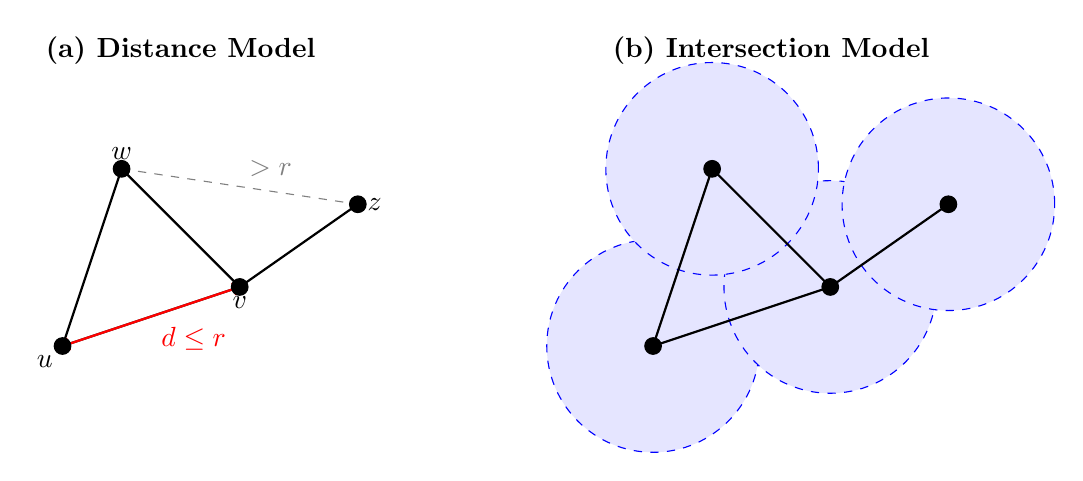
\begin{tikzpicture}[scale=1.5]
    % --- Pannello Sinistro: Distance Model ---
    \node at (1, 2.5) {\textbf{(a) Distance Model}};

    % definizione dei nodi (punti)
    \coordinate (A) at (0, 0);
    \coordinate (B) at (1.5, 0.5);
    \coordinate (C) at (0.5, 1.5);
    \coordinate (D) at (2.5, 1.2);

    % Disegno degli archi validi (distanza <= r)
    \draw[thick] (A) -- (B) -- (C) -- (A);
    \draw[thick] (B) -- (D);

    % Disegno di un arco non valido per mostrare che la distanza > r
    \draw[dashed, gray] (C) -- (D) node[midway, above right] {$> r$};

    % Etichetta della distanza <= r
    \draw[<->, red, thick] (A) -- (B) node[midway, below right] {$d \leq r$};

    % Disegno dei pallini dei nodi
    \filldraw (A) circle (2pt) node[below left] {$u$};
    \filldraw (B) circle (2pt) node[below] {$v$};
    \filldraw (C) circle (2pt) node[above] {$w$};
    \filldraw (D) circle (2pt) node[right] {$z$};

    % --- Pannello Destro: Intersection Model ---
    \begin{scope}[xshift=5cm] % Sposto tutto a destra di 5cm
    \node at (1, 2.5) {\textbf{(b) Intersection Model}};

    \coordinate (A2) at (0, 0);
    \coordinate (B2) at (1.5, 0.5);
    \coordinate (C2) at (0.5, 1.5);
    \coordinate (D2) at (2.5, 1.2);

    % Raggio dei cerchi (r/2)
    \def\rad{0.9}

    % Disegno i cerchi (le "aree di influenza")
    \draw[fill=blue!10, draw=blue, dashed] (A2) circle (\rad);
    \draw[fill=blue!10, draw=blue, dashed] (B2) circle (\rad);
    \draw[fill=blue!10, draw=blue, dashed] (C2) circle (\rad);
    \draw[fill=blue!10, draw=blue, dashed] (D2) circle (\rad);

    % Disegno gli archi dove i cerchi si sovrappongono
    \draw[thick] (A2) -- (B2) -- (C2) -- (A2);
    \draw[thick] (B2) -- (D2);

    \filldraw (A2) circle (2pt);
    \filldraw (B2) circle (2pt);
    \filldraw (C2) circle (2pt);
    \filldraw (D2) circle (2pt);
    \end{scope}
\end{tikzpicture}
\caption{The equivalent geometric representations of a Unit Disk Graph (UDG) adapted from \cite{CLARK1990165}. \textbf{(a)} The Distance Model connects nodes $u$ and $v$ if their Euclidean distance is $d \leq r$. \textbf{(b)} The Intersection Model places a disk of radius $r/2$ centered on each node; edges are formed exclusively where disks overlap.}
\label{fig:udg_models}
\end{figure}

Given any of these three definitions, the other two can be derived in linear time, demonstrating that they describe the exact same class of graphs. Historically, UDGs have proven to be an excellent mathematical framework for modeling broadcast and cellular networks, effectively resolving real-world problems such as frequency assignment and emergency signal routing \cite{CLARK1990165}. 

In the context of this thesis, the distance model is ''the elected'' model: replacing the generic threshold distance $r$ with the Rydberg radius ($R_b$) perfectly captures the physical interaction connectivity of neutral atoms in a quantum register.

As previously mentioned, the Maximum Independent Set (MIS) is a classic $NP$-Hard combinatorial optimization problem. While canonically formulated on general graphs, it holds massive relevance for our architecture because the problem famously remains $NP$-Hard even when restricted to Unit Disk Graphs \cite{CLARK1990165}.

Formally, given a graph $G = (V, E)$, an \textit{Independent Set} (IS) is defined as a subset of vertices $I \subseteq V$ such that no two vertices within $I$ are adjacent. Mathematically, this constraint translates to:
\begin{equation}
    \forall u, v \in I, \; u \neq v \implies \{u, v\} \notin E
\end{equation}
The MIS problem entails finding an independent set that contains the largest possible number of vertices; in other words, the objective is to maximize the cardinality $|I|$.

Given the aforementioned definitions, a straightforward and perfect isomorphism emerges between the abstract MIS problem on a UDG and the physical dynamics of neutral atom arrays. Specifically, the geometric threshold radius $r$ of the UDG corresponds directly to the Rydberg blockade radius ($R_b$). 

Consequently, the core mathematical constraint of the MIS problem, which strictly forbids selecting two adjacent vertices, is natively and physically enforced by the Rydberg blockade phenomenon, which prevents any two atoms within a distance $R_b$ from being simultaneously excited to the Rydberg state. 
Because of this perfect theoretical alignment, applying a global laser pulse designed to maximize the number of excited atoms in the 2D register forces the quantum many-body system to naturally evolve toward a ground state that inherently encodes the exact solution to the Maximum Independent Set of the corresponding geometric graph \cite{Henriet2020quantumcomputing}.
\begin{figure}[htbp]
\centering
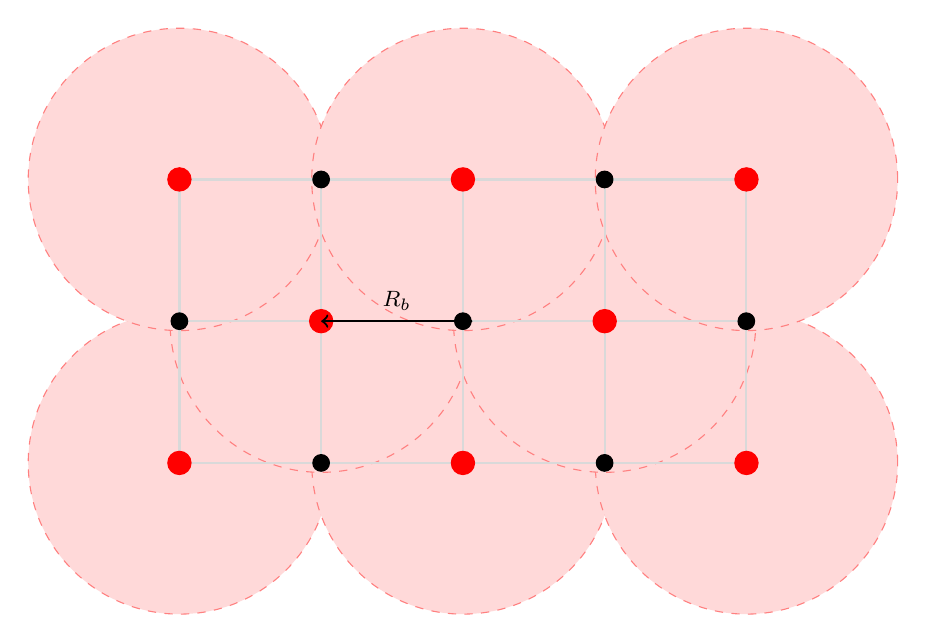
\begin{tikzpicture}[scale=1.2]
    
    % Definizione del Raggio di Rydberg (Rb) e spaziatura griglia
    \def\Rb{1.6}
    
    % Nodi della soluzione MIS (Atomi eccitati)
    \coordinate (E1) at (0,0);
    \coordinate (E2) at (3,0);
    \coordinate (E3) at (6,0);
    \coordinate (E4) at (1.5, 1.5);
    \coordinate (E5) at (4.5, 1.5);
    \coordinate (E6) at (0, 3);
    \coordinate (E7) at (3, 3);
    \coordinate (E8) at (6, 3);

    % Disegno prima i cerchi del blocco di Rydberg (sfumati in sottofondo)
    \foreach \p in {E1, E2, E3, E4, E5, E6, E7, E8} {
        \fill[red!15] (\p) circle (\Rb);
        \draw[red!50, dashed] (\p) circle (\Rb);
    }

    % Disegno gli archi del grafo UDG in modo corretto e nativo
    \draw[gray!30, thick, step=1.5] (0,0) grid (6,3);

    % Disegno tutti gli atomi neutri (Stato base, in nero)
    \foreach \x in {0, 1.5, 3, 4.5, 6} {
        \foreach \y in {0, 1.5, 3} {
            \filldraw[black] (\x,\y) circle (2.5pt);
        }
    }

    % Sovrascrivo gli atomi eccitati (Stato di Rydberg, in rosso e più grandi)
    \foreach \p in {E1, E2, E3, E4, E5, E6, E7, E8} {
        \filldraw[red] (\p) circle (3.5pt);
    }

    % Raggio 
    \draw[<->, thick] (E4) -- ++(\Rb,0) node[midway, above, font=\footnotesize] {$R_b$};

\end{tikzpicture}
\caption{Physical realization of the Maximum Independent Set (MIS) via the Rydberg blockade. Red dots represent atoms excited to the Rydberg state (\textbf{MIS selected nodes}), while black dots are atoms remained in the ground state (\textbf{unselected nodes}). 
The shaded red regions represent the Rydberg blockade volume (radius $R_b$). The physical mechanism preventing two Rydberg excitations from overlapping perfectly enforces the mathematical constraint of the MIS problem.}
\label{fig:rydberg_mis}
\end{figure}

\section{Literature and State of the Art}
\label{sec:SOTA}

Defining a definitive State of the Art (SOTA) for the embedding problem on neutral atom architectures is challenging, as the field remains at the absolute frontier of quantum computing research. Presently, there is no universally established protocol or singular ``gold standard'' architecture. Instead, the literature presents a diverse landscape of experimental approaches and heuristic strategies aimed at overcoming the strict geometric constraints of these platforms.

To illustrate this dynamic ecosystem, recent literature explores a wide array of embedding techniques. For instance, Vercellino et al. \cite{Vercellino_2022} investigate the use of Neural Networks to dynamically map problem graphs onto physical registers. Other approaches rely on force-directed heuristics; notably, Tarquini et al. \cite{tarquini2026dronedeliverypackingproblem} successfully (within a reasonable dimension less than circa 50 nodes) experimented with the Fruchterman-Reingold (FR) algorithm, enhanced by sophisticated pre- and post-processing techniques, 
to embed Quadratic Unconstrained Binary Optimization (QUBO) problems.

Alongside embedding algorithms, significant research is devoted to translating highly complex real-world use cases into physical layouts. Examples include the formulation of emergency hub placement routing \cite{tarquini2026emergencyhubplacementneutralatom} and satellite mission planning \cite{nowak2026satellitemissionplanningrydberg}, demonstrating the vast applicability of QUBO formulations on neutral atoms.


Most importantly for this thesis, several recent studies have started exploring advanced mapping and partitioning techniques as a workaround for hardware scale limitations. Works by Nembrini et al. \cite{nembrini2024application, Nembrini_2026} propose innovative Reinforcement Learning methodologies to tackle the severe embedding bottlenecks inherent to quantum annealing topologies. On the other hand, focusing strictly on neutral atom architectures, Das et al. \cite{das2025grid} explicitly propose problem partitioning, dividing the original combinatorial problem into sub-instances resolved using localized atomic arrays. While their specific methodologies differ from our scope, these partitioning strategies served as the foundational inspiration for the hybrid \textit{divide et impera} (divide and conquer) architecture proposed in the subsequent chapters of this work.

This diversity of approaches underscores the immaturity and the highly exploratory nature of the field. While the lack of rigid standards offers significant opportunities for novel theoretical contributions, it also introduces substantial experimental risks and engineering bottlenecks. 

Drawing from this extensive body of literature, we chose to restrict our focus specifically to the QUBO mathematical framework, which will be formally defined in the next section. More importantly, mainly driven by the operational realities and constraints of the currently available experimental platforms, our investigation will target QUBO instances that naturally exhibit a UDG-like connectivity. This specific focus bypasses the need for massive auxiliary embeddings, setting the optimal stage for our distributed algorithmic approach.


\section{Quadratic Unconstrained Binary Optimization (QUBO)}
\label{sec:QUBO}

Quadratic Unconstrained Binary Optimization (QUBO) provides a unifying mathematical framework for modeling a vast array of combinatorial optimization problems. As the name suggests, this formulation strictly involves binary decision variables and a quadratic objective function, notably without imposing any external algebraic constraints. 

This formulation has gained immense popularity across various scientific and industrial fields due to its remarkable versatility. As demonstrated in comprehensive tutorials \cite{glover2018tutorial}, a multitude of classically constrained problems (such as the TSP, Max-Cut, or Graph Coloring) can be seamlessly recast into the unconstrained QUBO format through the use of penalty terms. Consequently, a massive segment of modern literature focuses on QUBO as the standard input format for quantum platforms. While historically popularized by quantum annealing systems built on superconducting qubits (such as D-Wave \cite{QUBO-D-Wave}), QUBO is increasingly becoming the target formulation for neutral atom architectures as well \cite{nowak2026satellitemissionplanningrydberg, Vercellino_2022, das2025grid}.

From a formal mathematical perspective, solving a QUBO problem entails finding the specific assignment of a binary vector $x$ that minimizes (or maximizes, note that a minimization problem is equivalent to a maximization one by simply applying a minus sign ($-$) to the objective function) a quadratic cost function:

\begin{equation}
    \min_{x \in \{0,1\}^n} f(x) = x^T Q x = \sum_{i=1}^{n} \sum_{j=1}^{n} Q_{i,j} x_i x_j
\end{equation}

where:
\begin{itemize}
    \item $x = (x_1, x_2, \dots, x_n)$ is a vector of $n$ binary decision variables;
    \item $Q$ is an $n \times n$ square matrix of real constants detailing the problem's costs and interactions.
\end{itemize}

A key mathematical property of binary variables is that $x_i^2 = x_i$ for any $x_i \in \{0,1\}$. This elegantly allows any linear term of the objective function to be mapped directly onto the main diagonal of the $Q$ matrix ($Q_{i,i}$), while the off-diagonal elements ($Q_{i,j}$ for $i \neq j$) encode the quadratic interactions, or "penalties," between pairs of variables.

Our decision to adopt the QUBO framework for investigating hybrid embedding methodologies is twofold. First, it ensures broad applicability across the wide variety of problems identifiable in the literature \cite{glover2018tutorial}. Second, and most crucially, the binary nature of the variables establishes a native, one-to-one mapping with the physical states of a quantum register: each variable $x_i \in \{0,1\}$ directly dictates whether a specific atom $i$ is left in the ground state ($|0\rangle$) or excited to the Rydberg state ($|1\rangle$). This elegant bridge between mathematical abstraction and hardware execution perfectly sets the stage for the algorithmic development detailed in the next chapter.

\paragraph{Investigated QUBO Instances}
Due to specific hardware and simulator constraints, the experimental phase of this work focuses exclusively on UDG-like QUBO matrices. Specifically, we evaluate randomly generated QUBO instances whose underlying interaction connectivity strictly mirrors the geometric topology of a Unit Disk Graph.

Furthermore, to ensure physical compatibility with current neutral atom platforms, these matrices are constrained to exhibit uniform parameter distributions. All elements on the principal diagonal are assigned identical values; mathematically, this uniform linear cost reflects the hardware limitation of employing a global driving laser, which applies the same detuning and Rabi frequency uniformly across the entire atomic register. Similarly, all non-zero off-diagonal elements share a constant penalty value, effectively representing the uniform, binary nature of the Rydberg blockade interaction across all valid UDG edges.

